\documentclass[11pt]{article}

\usepackage[margin=1in]{geometry}
\usepackage{amsmath,amssymb,graphicx,multicol,array,enumerate,textcomp}
\usepackage{tikz}
\usepackage{pgfplots}
\pgfplotsset{compat=1.18}
\usetikzlibrary{arrows.meta,calc}

\usepgfplotslibrary{groupplots}
\newcommand{\usd}{\text{\$}}
\newenvironment{problem}[2][Problem]{\begin{trivlist}
\item[\hskip \labelsep {\bfseries #1}\hskip \labelsep {\bfseries #2.}]
\leavevmode\par
}{\end{trivlist}}

% ---- Small style helpers (match lecture-style look) ----
\definecolor{mmdred}{RGB}{200,50,50}
\definecolor{msblue}{RGB}{70,110,200}
\definecolor{fxgreen}{RGB}{40,150,90}
\definecolor{retorange}{RGB}{230,140,40}
\definecolor{graydash}{RGB}{120,120,120}

\begin{document}

\title{Problem Set 3: Asset Model}
\author{Joe White\\ECO 442}
\date{\today}
\maketitle

\begin{problem}{1}

\begin{enumerate}[(a)]
\item \textbf{Policy to raise interest rates in Costa Rica.}

Money market equilibrium is
\[
MS = MD
\quad\Longleftrightarrow\quad
\frac{MS}{P} = L(R_C,Y_C),
\]
where $R_C$ is the Costa Rican interest rate.
In the short run $P$ is fixed, so to increase $R_C$ we have to decrease the real money supply $\frac{MS}{P}$. Meaning we implement a contractionary monetary policy: $MS\downarrow$.

\vspace{0.25em}

% ---------- Money Market Figure (ylabel moved left, correct orientation) ----------
\begin{center}
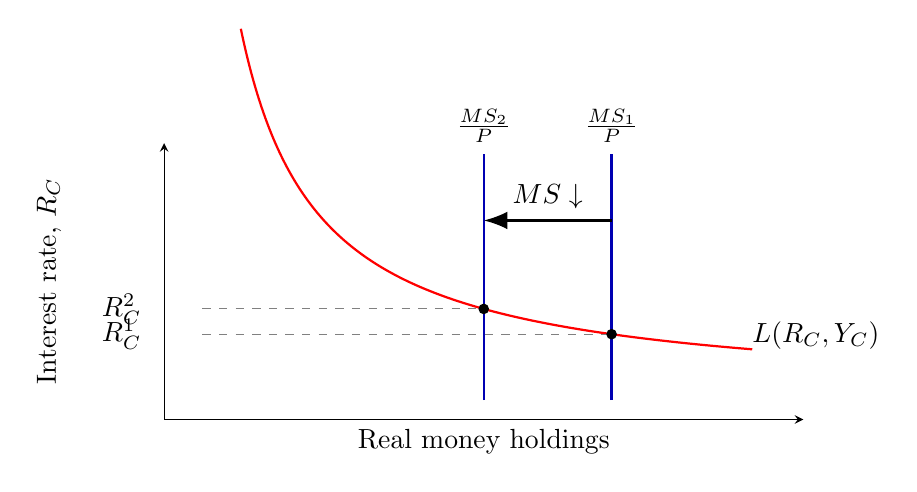
\begin{tikzpicture}
\begin{axis}[
  width=0.80\textwidth,
  height=0.42\textwidth,
  axis lines=left,
  xmin=0, xmax=10,
  ymin=0, ymax=10,
  xtick=\empty, ytick=\empty,
  xlabel={Real money holdings},
  ylabel={Interest rate, $R_C$},
  xlabel style={yshift=2pt},
  ylabel style={
    at={(axis description cs:-0.18,0.50)}, % move left (negative x)
    anchor=center
  },
  clip=false
]

\def\A{16}
\def\B{0.8}

\addplot[red, thick, domain=1.2:9.2, samples=250]
  ({x},{\A/x + \B});

\node[anchor=west] at (axis cs:9.05,3.05) {$L(R_C,Y_C)$};

\def\xone{7.0}
\def\xtwo{5.0}

\addplot[blue!70!black, thick] coordinates {(\xone,0.7) (\xone,9.6)};
\node[anchor=south] at (axis cs:\xone,9.65) {$\frac{MS_1}{P}$};

\addplot[blue!70!black, thick] coordinates {(\xtwo,0.7) (\xtwo,9.6)};
\node[anchor=south] at (axis cs:\xtwo,9.65) {$\frac{MS_2}{P}$};

\pgfmathsetmacro{\Rone}{\A/\xone + \B}
\pgfmathsetmacro{\Rtwo}{\A/\xtwo + \B}

\addplot[black, only marks, mark=*, mark size=1.7pt] coordinates {(\xone,\Rone)};
\addplot[black, only marks, mark=*, mark size=1.7pt] coordinates {(\xtwo,\Rtwo)};

\addplot[gray, dashed] coordinates {(0.6,\Rone) (\xone,\Rone)};
\addplot[gray, dashed] coordinates {(0.6,\Rtwo) (\xtwo,\Rtwo)};

\node[anchor=east] at (rel axis cs:-0.02,{\Rone/10}) {$R_C^{1}$};
\node[anchor=east] at (rel axis cs:-0.02,{\Rtwo/10}) {$R_C^{2}$};

\draw[-{Latex[length=3mm]}, thick] (axis cs:\xone,7.2) -- (axis cs:\xtwo,7.2);
\node[anchor=south] at (axis cs:{(\xone+\xtwo)/2},7.25) {$MS \downarrow$};

\end{axis}
\end{tikzpicture}
\end{center}

So the policy of decreasing the supply of col\'ons $(MS \downarrow)$ raises the interest rate $(R_C \uparrow)$.

\item \textbf{Effect on the Col\'on/USD exchange rate.}

For a Costa Rican investor comparing col\'on deposits vs.\ dollar deposits, uncovered IRP is
\[
\frac{1+i_C}{1+i_\$} \;=\; \frac{E^{1YR}_{C/\$}}{E_{C/\$}}.
\]
Holding $i_{\usd}$, $E^{1YR}_{C/\usd}$ constant, if $i_C\uparrow$ then the left-hand side rises, so $\frac{E^{1YR}_{C/\$}}{E_{C/\$}}$ must rise; with $E^{1YR}_{C/\$}$ fixed this requires $E_{C/\$}\downarrow$.

Meaning the col\'on appreciates against the dollar in the short run:
\[
E_{C/\$}\downarrow \quad\Longleftrightarrow\quad \text{fewer col\'on s per \$1}.
\]

\vspace{0.25em}

% ---------- IRP Figure (tick labels outside + clearer curve labels) ----------
\begin{center}
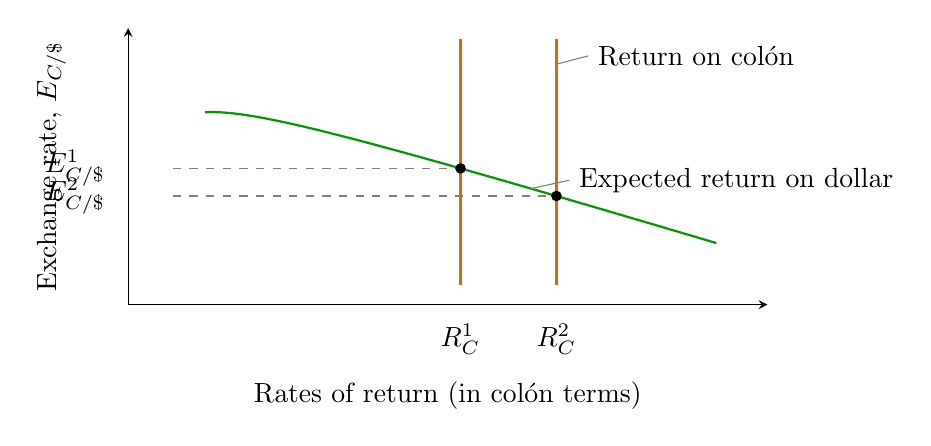
\begin{tikzpicture}
\begin{axis}[
  width=0.80\textwidth,
  height=0.42\textwidth,
  axis lines=left,
  xmin=0, xmax=10,
  ymin=0, ymax=10,
  xtick=\empty, ytick=\empty,
  xlabel={Rates of return (in col\'on\ terms)},
  ylabel={Exchange rate, $E_{C/\usd}$},
  % move axis titles to match outside labels
  xlabel style={yshift=-22pt},
  ylabel style={
    at={(axis description cs:-0.12,0.50)}, % slight left shift like your first graph
    anchor=center
  },
  clip=false
]

% Expected return on dollar deposits (green curve)
\addplot[green!60!black, thick, domain=1.2:9.2, samples=250]
  ({x},{8.8 - 0.7*x - 1.2/x});

% Return on colón deposits (orange vertical lines)
\def\Rcxone{5.2}
\def\Rcxtwo{6.7}
\addplot[orange!85!black, very thick] coordinates {(\Rcxone,0.7) (\Rcxone,9.6)};
\addplot[orange!85!black, very thick] coordinates {(\Rcxtwo,0.7) (\Rcxtwo,9.6)};

% Intersections (dots)
\pgfmathsetmacro{\Eone}{8.8 - 0.7*\Rcxone - 1.2/\Rcxone}
\pgfmathsetmacro{\Etwo}{8.8 - 0.7*\Rcxtwo - 1.2/\Rcxtwo}

\addplot[black, only marks, mark=*, mark size=1.7pt] coordinates {(\Rcxone,\Eone)};
\addplot[black, only marks, mark=*, mark size=1.7pt] coordinates {(\Rcxtwo,\Etwo)};

% Dashed horizontal guides
\addplot[gray, dashed] coordinates {(0.7,\Eone) (\Rcxone,\Eone)};
\addplot[gray, dashed] coordinates {(0.7,\Etwo) (\Rcxtwo,\Etwo)};

% ---- Put E^1 and E^2 labels LEFT of the y-axis (outside)
\node[anchor=east] at (rel axis cs:-0.02,{\Eone/10}) {$E^{1}_{C/\usd}$};
\node[anchor=east] at (rel axis cs:-0.02,{\Etwo/10}) {$E^{2}_{C/\usd}$};

% ---- Put R_C^1 and R_C^2 labels BELOW the x-axis (outside)
\node[anchor=north] at (rel axis cs:{\Rcxone/10},-0.035) {$R_C^{1}$};
\node[anchor=north] at (rel axis cs:{\Rcxtwo/10},-0.035) {$R_C^{2}$};

% ---- Clear labels with leader lines
% Label for green curve
\node[anchor=west] (dolLab) at (axis cs:6.9,4.5) {Expected return on dollar};
\draw[gray] (dolLab.west) -- (axis cs:6.3,{8.8 - 0.7*6.3 - 1.2/6.3});

% Label for orange lines (attach to the right line)
\node[anchor=west] (colLab) at (axis cs:7.2,9.0) {Return on col\'on};
\draw[gray] (colLab.west) -- (axis cs:\Rcxtwo,8.7);

\end{axis}
\end{tikzpicture}
\end{center}

Holding $i_{\$}$ and $E^{1YR}_{C/\$}$ constant, an increase in the Costa Rican interest rate implies
\[
i_C \uparrow \ \Rightarrow\ E_{C/\$}\downarrow \ \Rightarrow\ \text{the col\'on appreciates in the short run.}
\]

\item \textbf{Effect on probability a Costa Rican consumer buys a car produced in Costa Rica.}

We changed policy by reducing $MS$, which raises the Costa Rican interest rate $R_C$. Under the short-run assumption, prices in col\'on s are fixed, so the price of the Costa Rican car in col\'on s is unchanged in the short run.

Higher $R_C$ increases borrowing costs and reduces the amount of financing households can obtain.
Therefore the probability of purchasing the car falls:
\[
MS\downarrow \Rightarrow R_C\uparrow \Rightarrow \text{Probability of buying CR car}\downarrow.
\]

\item \textbf{Effect on probability a U.S.\ consumer buys a Costa Rican car sold in the U.S.}

From part (b), the col\'on appreciates. Meaning one col\'on is worth more dollars, so Costa Rican goods become more expensive in dollars. The U.S.\ dollar price of a Costa Rican-produced car rises, lowering the probability a U.S.\ consumer buys it.

Holding U.S.\ interest rates fixed (since this policy is in Costa Rica):
\[
\text{col\'on appreciation} \Rightarrow \text{CR goods in \$ become more expensive} \Rightarrow \text{Probability of buying CR car}\downarrow.
\]
\end{enumerate}
\end{problem}

\begin{problem}{2}

Money demand is $MD = P\cdot L(R_C,Y_C)$, so an increase in income shifts $L(R_C,Y_C)$ outward:
\[
Y_C\uparrow \quad\Rightarrow\quad L(R_C,Y_C)\ \text{increases.}
\]
With prices fixed and $MS$ unchanged, money market equilibrium
\[
\frac{MS}{P}=L(R_C,Y_C)
\]
requires a higher interest rate to reduce real money demand back to the fixed supply. So:
\[
Y_C\uparrow \Rightarrow L(R_C,Y_C)\uparrow \Rightarrow R_C\uparrow.
\]

From IRP,
\[
\frac{1+i_C}{1+i_\$}=\frac{E^{1YR}_{C/\$}}{E_{C/\$}},
\]
holding $i_{\usd}$, $E^{1YR}_{C/\usd}$ constant, $i_C\uparrow$ implies $E_{C/\usd}\downarrow$ (col\'on appreciation).

% ---------- Combined Asset Model (side-by-side, aligned, with outside tick labels) ----------
% Preamble needs:
% \usepackage{tikz}
% \usepackage{pgfplots}
% \pgfplotsset{compat=1.18}
% \newcommand{\usd}{\text{\$}}

\begin{center}
\makebox[\textwidth]{%
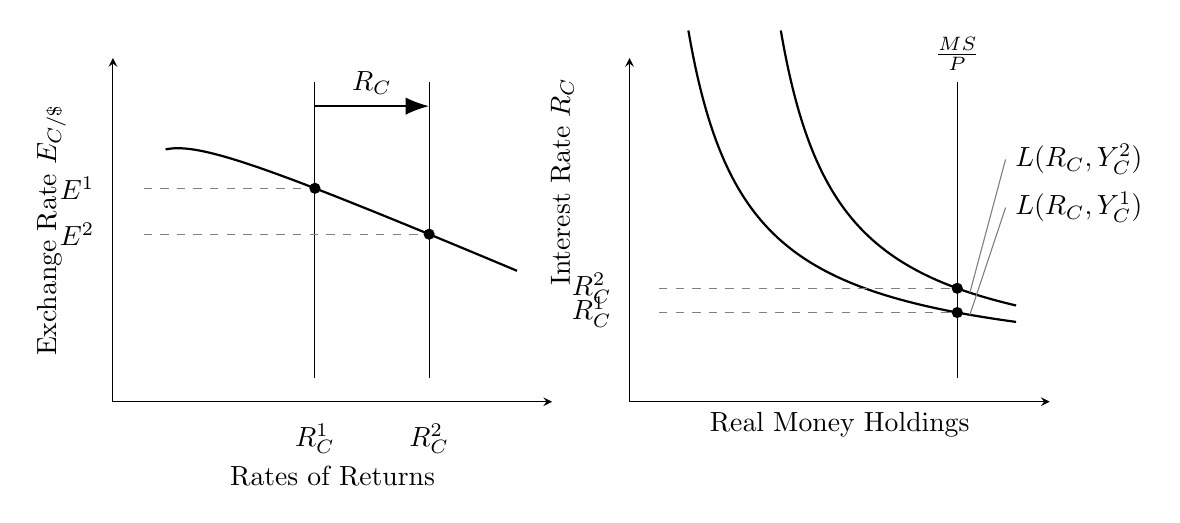
\begin{tikzpicture}

% =========================
% LEFT PANEL: FX / IRP
% =========================
\begin{axis}[
  name=fx,
  width=0.46\textwidth,
  height=0.36\textwidth,
  scale only axis,
  axis lines=left,
  xmin=0, xmax=10,
  ymin=0, ymax=10,
  xtick=\empty, ytick=\empty,
  xlabel={Rates of Returns},
  ylabel={Exchange Rate $E_{C/\usd}$},
  % move axis titles to make room for outside labels
  xlabel style={at={(axis description cs:0.50,-0.16)}, anchor=north},
  ylabel style={at={(axis description cs:-0.14,0.50)}, anchor=center},
  clip=false
]

% Downward-sloping curve
\addplot[black, thick, domain=1.2:9.2, samples=300]
  ({x},{9.0 - 0.55*x - 1.2/x});

% Two vertical lines at R_C^1 and R_C^2
\def\RcOne{4.6}
\def\RcTwo{7.2}
\addplot[black] coordinates {(\RcOne,0.7) (\RcOne,9.3)};
\addplot[black] coordinates {(\RcTwo,0.7) (\RcTwo,9.3)};

% Points on curve
\pgfmathsetmacro{\Eone}{9.0 - 0.55*\RcOne - 1.2/\RcOne}
\pgfmathsetmacro{\Etwo}{9.0 - 0.55*\RcTwo - 1.2/\RcTwo}
\addplot[black, only marks, mark=*, mark size=1.8pt] coordinates {(\RcOne,\Eone)};
\addplot[black, only marks, mark=*, mark size=1.8pt] coordinates {(\RcTwo,\Etwo)};

% Dashed horizontals
\addplot[gray, dashed] coordinates {(0.7,\Eone) (\RcOne,\Eone)};
\addplot[gray, dashed] coordinates {(0.7,\Etwo) (\RcTwo,\Etwo)};

% ---- Outside labels (like your single graphs)
\node[anchor=east]  at (rel axis cs:-0.02,{\Eone/10}) {$E^{1}$};
\node[anchor=east]  at (rel axis cs:-0.02,{\Etwo/10}) {$E^{2}$};
\node[anchor=north] at (rel axis cs:{\RcOne/10},-0.035) {$R_C^{1}$};
\node[anchor=north] at (rel axis cs:{\RcTwo/10},-0.035) {$R_C^{2}$};

% Arrow showing move from R_C^1 to R_C^2
\draw[-{Latex[length=3mm]}, thick] (axis cs:\RcOne,8.6) -- (axis cs:\RcTwo,8.6);
\node[anchor=south] at (axis cs:{(\RcOne+\RcTwo)/2},8.65) {$R_C$};

\end{axis}

% =========================
% RIGHT PANEL: MONEY MARKET (fit + ylabel moved above outside labels)
% =========================
\begin{axis}[
  name=mm,
  at={(fx.north east)}, anchor=north west, xshift=28pt, % smaller gap to help fit
  width=0.44\textwidth,   % slightly narrower so nothing spills
  height=0.36\textwidth,
  scale only axis,
  axis lines=left,
  xmin=0, xmax=10,
  ymin=0, ymax=10,
  xtick=\empty, ytick=\empty,
  xlabel={Real Money Holdings},
  ylabel={Interest Rate $R_C$},
  xlabel style={yshift=2pt},
  % Put ylabel UP and LEFT so it clears the R_C^1, R_C^2 labels:
  ylabel style={
    at={(axis description cs:-0.16,0.64)}, % left of axis and higher
    anchor=center
  },
  clip=false
]

\def\A{14}
\def\B{0.8}
\def\Delta{2.2}
\def\xMS{7.8}

% Money supply
\addplot[black] coordinates {(\xMS,0.7) (\xMS,9.3)};
\node[anchor=south] at (axis cs:\xMS,9.35) {$\frac{MS}{P}$};

% Money demand curves
\addplot[black, thick, domain=1.4:9.2, samples=300]
  ({x},{\A/x + \B});
\addplot[black, thick, domain={1.4+\Delta}:9.2, samples=300]
  ({x},{\A/(x-\Delta) + \B});

% Equilibria
\pgfmathsetmacro{\RoneMM}{\A/\xMS + \B}
\pgfmathsetmacro{\RtwoMM}{\A/(\xMS-\Delta) + \B}
\addplot[black, only marks, mark=*, mark size=1.8pt] coordinates {(\xMS,\RoneMM)};
\addplot[black, only marks, mark=*, mark size=1.8pt] coordinates {(\xMS,\RtwoMM)};

% Dashed guides
\addplot[gray, dashed] coordinates {(0.7,\RoneMM) (\xMS,\RoneMM)};
\addplot[gray, dashed] coordinates {(0.7,\RtwoMM) (\xMS,\RtwoMM)};

% Outside labels (left of y-axis)
\node[anchor=east] at (rel axis cs:-0.02,{\RoneMM/10}) {$R_C^{1}$};
\node[anchor=east] at (rel axis cs:-0.02,{\RtwoMM/10}) {$R_C^{2}$};

% L-labels pulled slightly inward so they don't overflow the page
\node[anchor=west] (L2) at (axis cs:8.95,7.05) {$L(R_C,Y_C^{2})$};
\draw[gray] (L2.west) -- (axis cs:8.10,{\A/(8.10-\Delta)+\B});

\node[anchor=west] (L1) at (axis cs:8.95,5.65) {$L(R_C,Y_C^{1})$};
\draw[gray] (L1.west) -- (axis cs:8.10,{\A/8.10+\B});

\end{axis}

\end{tikzpicture}
}%
\end{center}

So in the short-run:
\[
Y_C\uparrow \Rightarrow MD\uparrow \Rightarrow R_C\uparrow
\Rightarrow E_{C/\$}\downarrow \ (\text{col\'on appreciation}).
\]
\end{problem}

\end{document}